\documentclass{swp}
\usepackage{hyperref}
\usepackage{amsmath}
\usepackage{amssymb}

\begin{document}

\maketitle{Entwurfsbeschreibung Gesamtprojekt}{15.09.2015}{Paul Eisenhuth}
\\\\\\\\\\

\tableofcontents
%\newpage
\section{Allgemeines}
Die Stadtteilplattform Leipziger Osten soll mit umfangreichen Funktionen ausgestattet sein, um gute Nutzbarkeit zu gew\"ahrleisten. Akteure haben hier die M\"oglichkeit, ein \"offentliches Profil zu erstellen, ihre Veranstaltungen einzutragen und auf einer anschaulichen Karte und einem Terminkalender mit vielen Filterfunktionen der \"Offentlichkeit anzeigen zu lassen. Dadurch soll der Stadtteil Leipziger Osten attraktiver gemacht und Bausteine f\"ur Synergien einzelner Akteure gebildet werden. Diese grundlegende Struktur der Plattform wird auf Basis von Drupal realisiert. Dies erm\"oglicht einen einfachen Ausbau der Webseite mittels Modulen, die f\"ur Drupal zu Verf\"ugung stehen, wobei s\"amtliche Kernfunktionen von einem eigens daf\"ur entwickelten Modul und Theme realisiert werden.\\
Die Plattform entsteht in Zusammenarbeit mit Matthias Petzold von leipziger-ecken.de.
\subsection{Installationsanleitung}
Drupal muss auf einem Webserver installiert werden. Anweisungen hierf\"ur sind unter \url{https://www.drupal.org/documentation/install} zu finden. Es wird ein eigenst\"andiges Modul (aae\_{}data) und Thema (aae\_{}theme) entwickelt, so dass diese lediglich in den entsprechenden Drupal-Ordner kopiert und via Backend aktiviert werden m\"ussen. Dabei wird die Datenstruktur in die Datenbank importiert, sowie Inhalte (Bezirke von Leipzig) in die Datenbank geschrieben. \\
Detaillierte Anweisungen k\"onnen der separaten Installationsanleitung entnommen werden.
\subsection{Backupkonzept}
Um ein sicheres Arbeiten zu gew\"ahrleisten, wird nicht auf der Drupalinstanz des Servers gearbeitet. Jedes Teammitglied installiert sich eine eigene Drupalinstanz auf seinem lokalen Arbeitsrechner. Der Kern, d.h. Originalthemes und -module, werden nicht ver\"andert.  Das bearbeitete Modul und das Theme werden \"uber das git-Repository verwaltet und in Drupal verlinkt, so dass Fehlschl\"age r\"uckg\"angig gemacht werden k\"onnen.
\section{Produkt\"ubersicht}
Die Stadtteilplattform bietet Akteuren (Vereinen, Initiativen, ...) aus Leipzig (vorerst jedoch Konzentration auf den Osten) eine Pr\"asentationsm\"oglichkeit. Hierf\"ur k\"onnen sie ein \"offentliches Profil anlegen. Ein \"offentliches Profil beinhaltet zentrale Informationen zum Akteur (Name, Adresse, E-Mail, Webseite, Telefonnummer, Beschreibung, \"Offnungszeiten, Bild).\\
Desweiteren gibt es die M\"oglichkeit Veranstaltungen einzutragen. Events werden auf einer eigenen Seite dargestellt. Diese beinhaltet Name, Webseite, Datum, Ort, Sparte, Beschreibung,  sowie eine Verkn\"upfung zum \"offentlichen Profil des Akteurs (falls erw\"unscht). Die Events werden in einem Veranstaltungskalender angezeigt und k\"onnen im iCal-Format heruntergeladen werden.\\
Neuigkeiten und Informationen \"uber Leipzigrelevante Theme k\"onnen Redakteure im Journal (Blog) ver\"offentlichen. Diese Beitr\"age bestehen aus einem Titel, Text und Bild.\\
Eine Karte zeigt den Leipziger Osten und soll in K\"urze auch Akteure und Veranstaltungen anzeigen und interaktiv erkundbar machen.\\
Genauere Beschreibungen aller Funktionalit\"aten sind im separaten Handbuch einzusehen.
\section{Grunds\"atzliche Struktur- und Entwurfsprinzipien}
\subsection{Schichtenmodell}
Aufgeteilt ist die Stadtteilplattform in 3 Schichten. Die grafische Benutzeroberfl\"ache im Webbrowser stellt die Clientschicht dar. Auf dem Server befinden sich zwei weitere Schichten: die Datenschicht in Form einer MySql-Datenbank und die Funktionsschicht, welche die Skripte enth\"alt und von Drupal realisiert wird.
\subsection{Arbeitsteilung}
Das Team arbeitet in der Implementierungsphase in kleineren Gruppen, um eine parallele aber personell m\"oglichst getrennte Entwicklung von Layout, Backend, und Datenstruktur zu erm\"oglichen.
\subsubsection{Layout}
Der/die Layouter sind mit der Gestaltung der Plattform und ihrer interaktiven Elemente betraut und entwickeln ein eigenes Drupal-Theme. Das Layout wird fortschreitend mit den anderen Ebenen der Plattform entwickelt, um auf eventuelle \"Anderungen von deren Seiten aus reagieren zu k\"onnen. 
\subsubsection{Backend}
Die Backend-Gruppe ist f\"ur die Installation, das Einrichten der Drupal-Instanz verantwortlich. In der Implementierungsphase arbeitet dieser Teil des Teams an der Entwicklung eines eigenen Drupal-Moduls und der Verkn\"upfung aller Module und Funktionalit\"aten des Systems.
\subsubsection{Daten}
Eine weitere Gruppe ist f\"ur die Entwicklung des Datenbankschemas zust\"andig.
\section{Struktur- und Entwurfsprinzipien einzelner Pakete}
\subsection{Darstellungsebene}
Es soll eine Hauptseite geben, die die interaktive Karte, den Kalender, Snippets von Akteurprofilen und eine Navigationsleiste beinhaltet. Weiterhin soll es Seiten geben f\"ur: Akteurprofile, Events, den Kalender, die Registrierung, die Karte, FAQ und Journal, \"Uber uns, Impressum.
\subsection{Eigenes Drupal-Modul}
Im Modul aae\_{}data werden s\"amtliche Ebenen des Backends umgesetzt. Es werden Datenbanktabellen angelegt, sowie ben\"otigte Daten in die Datenbank geschrieben. Desweiteren werden alle erforderlichen Seiten gebaut und in Drupal integriert. Diese werden durch einzelne PHP-Skripte generiert. Dieses ist fest mit dem aae\_{}theme Theme verkn\"upft.
\subsection{Eigenes Drupal-Theme}
Um bei der Gestaltung des Layouts freie Hand zu haben und eigene Ideen umsetzen zu k\"onnen, wird f\"ur die Stadtteilplattform ein eigenes Drupal-Theme entwickelt: aae\_{}theme. Dieses ist fest mit dem aae\_{}data Modul verkn\"upft.\\
Das Theme ist responsive.
\section{Datenmodell}
Das Datenmodell basiert auf den Anforderungen der Initiative leipziger-ecken.de:\\\\
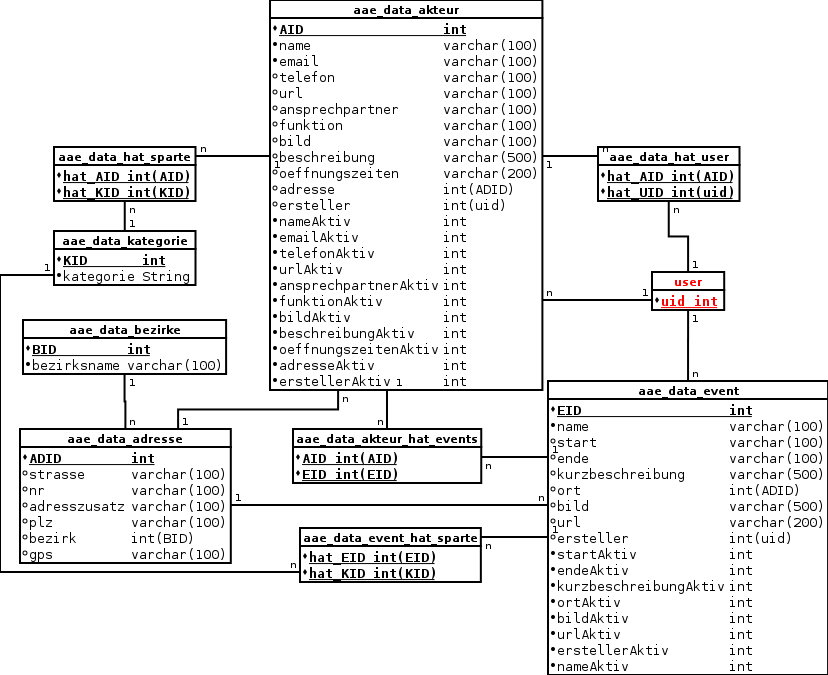
\includegraphics[width=\textwidth]{Datenmodell7.png}
\section{Testkonzept}
Um in der Implementierungsphase effizient arbeiten zu k\"onnen, d\"urfen die Tests selbst nicht unn\"otig viel Zeit in Anspruch nehmen. Aufgrund von sehr beschr\"ankten personellen Ressourcen wurden mit Ausnahme von manuellen \"Uberpr\"ufungen der Komponenten und deren Integration Tests an das Team von leipziger-ecken.de ausgelagert.\\
Demnach wurden im Rahmen des Projekts bisher lediglich manuelle Systemtests auf dem Praktikumsserver durchgef\"uhrt, sowie ein laufender Alphatest mit Akteuren und Redakteuren des Leipziger Ostens.
\section{Glossar}
Stadtteilplattform: \\Eine interaktive (Online)-Plattform, welche der Organisation, Versch\"onerung, Attraktivit\"at, Vermittlung, \glqq News-Verbreitung\grqq{} und vielem mehr dienen soll. Die Plattform sollte so aufgesetzt sein, dass sie in gewisser Weise selbst fuktioniert und mit Inhalten bespielt wird. Das hei{\ss}t Nutzer k\"onnen sich registrieren, f\"ur im Viertel aktive Akteure \"offentliche Profile anlegen und \"uber diese Veranstaltungen und Angebote ver\"offentlichen, ohne dass alles von einem Betreiber der Seite im Voraus einzeln kontrolliert werden muss. Aus inhaltlichen, gesetzlichen, datenschutzrechtlichen Gr\"unden kann eine Nachmoderation, siehe \glqq Nutzer\grqq{}/\glqq Seitenbetreiber\grqq{}). Ziel der Plattform ist es, eine \"ubersichtliche Website zu gestalten, die mittels Interaktiver Karte, Kalender, etc. den Stadtteil mit seinen Akteuren attraktiv macht.

Nutzer:\\Nutzer sind zun\"achst jegliche Besucher der Plattform, die diese zu Informations- und Pr\"asentationszwecken nutzen. Auch alle anderen auf der Plattform aktiven Menschen (z.B. von Betreiberseite) k\"onnen zus\"atzlich in der Rolle des Nutzer auf ihr unterwegs sein. Nutzer k\"onnen alle \"offentlichen Seiten der Plattform aufrufen.\\ 
Nutzer haben zus\"atzlich die M\"oglichkeit, sich auf der Plattform mit einem eigenen Account zu registrieren. Dies erm\"oglicht ihnen das Anlegen eines \"offentlichen Profils f\"ur einen im Stadtteil aktiven Akteur, den der Nutzer auch im realen Leben vertritt. Dies muss im Zweifelsfall von den Seitenbetreibern \"uberpr\"uft und verifiziert werden.

Akteur:\\
Unter Akteuren sind zun\"achst Folgende zu verstehen: Veranstalter, Vereine, Initiativen und Privatpersonen, die im Leipziger Osten auf verschiedene Art aktiv sind. Im Rahmen der Architektur unserer Plattform bezeichnet \glqq Akteur\grqq{} auch die Repr\"asentation einer solchen Institution, die online von einem oder mehreren Nutzern, die der Institution auch in der realen Welt angeh\"oren, (Akteursinhaber \& Akteursmitglieder) vertreten und verwaltet wird. Die \"offentliche Repr\"asentation eines Akteurs auf der Plattform ist das zugeh\"orige Akteursprofil.

Akteursinhaber/Akteursadmin:\\Registrierter Nutzer, der f\"ur einen realweltlichen Akteur ein \"offentliches Profil auf der Stadtteilplattform anlegt, und f\"ur dieses Administratorrechte besitzt. Diese umfassen vollst\"andige Bearbeitungsrechte f\"ur die Inhalte des Profils (ausgenommen Moderation von Nutzerkommentaren), sowie das Recht die L\"oschung des Profils vorzunehmen, bzw. zu veranlassen, oder den Adminstatus an einen anderen registrierten Nutzer oder die Plattformbetreiber abzugeben.

Akteursmitglied:\\Das \"offentliche Profil eines Akteurs soll auch von mehreren Personen verwaltbar sein. Akteursmitglieder sind registrierte Nutzer, denen vom Akteursadmin beschr\"ankte Bearbeitungsrechte zugewiesen wurden. Diese k\"onnen beispielsweise die Bearbeitung von (bestimmten) Inhalten einschlie{\ss}en, aber Akteursmitgliedern keine L\"oschung des Profils zu erm\"oglichen.

Akteursprofil / Kurzdarstellung:\\Von Nutzern verwaltete Selbstdarstellung von Akteuren auf der Stadtteilplattform, \"ahnlich eines Profils in sozialen Netzwerken. Dieses sollte mindestens folgende Daten umfassen: Name, Beschreibung, Adresse, sonstige Kontaktm\"oglichkeit (E-Mail, Facebook...), Sparte, Zielgruppe. Optional sind Bilder, etc. Um ein Profil f\"ur einen Akteur auf der Plattform anzulegen, ben\"otigen die ihm zugeh\"origen Nutzer eine entsprechende Zugangsm\"oglichkeit \"uber einen registrierten Account.

Seitenbetreiber:\\Inhaber und Betreiber der Stadtteilplattform, insbesondere nach \"Ubergabe des Projekts. Der Seitenbetreiber kann eine Person oder eine Institution, z.B. ein Verein sein. In der Praxis k\"onnen im Seitenbetreiber auch verschiedene administrative Aufgaben vereint sein, beispielsweise technische Administration, Nutzerverwaltung, sowie Moderation und redaktionelle T\"atigkeiten. Eine andere personelle und inhaltliche Verteilung der administrativen Aufgaben ist ebenfalls denkbar.

Redakteure:\\Registrierter Nutzer, welcher Schreibrecht f\"ur das Journal besitzt und dort Artikel ver\"offentlichen kann.

Journal:\\Blog, welcher von Redakteuren bearbeitet werden kann.

\end{document}
